\documentclass[11pt,a4paper]{article}
\usepackage[T1]{fontenc}
\usepackage[margin=2.3cm]{geometry}
\usepackage{amsmath,amssymb}
\usepackage{graphicx}
\usepackage[dvipsnames]{xcolor}
\usepackage{enumitem}
\usepackage[colorlinks=true,linkcolor=blue,urlcolor=blue]{hyperref}
\setlength{\parskip}{0.6em}
\setlength{\parindent}{0pt}
\begin{document}

\begin{center}{\LARGE\bfseries opencncpath}\\[0.4em]{\large Turn a drawing into a CNC toolpath, in five sessions.}\\[0.2em]\small PAN IIT OSS explainer \textbullet{} diploma / undergraduate to advanced undergraduate (levels 5-6)\end{center}

\section*{Why this exists}
Every machined part starts as a drawing and ends as a list of coordinates that a cutter follows. This explainer shows the geometry in between, offsets, arcs, stepovers and a height-map check, using only simple formulas, so you can build it yourself.

\section*{The end goal}
Turn a drawing into a CNC toolpath. The end goal is to turn a drawing into a CNC toolpath: the planning step that CAM software does for machining. This repo teaches the geometry only; real machining needs trained operators, machine-specific post-processing and safety checks.

\section*{How the five sessions build up}
\begin{enumerate}[nosep]
\item \textbf{Session 1: A cutter follows a path} (Level 1, conceptual interactive model, 60 min).
\item \textbf{Session 2: G-code, offsets and arcs} (Level 2, mathematical engineering model, 75 min).
\item \textbf{Session 3: Pocketing strategies and a simulation that checks them} (Level 3, simulation and validation, 90 min).
\item \textbf{Session 4: Offset any convex polygon} (Level 3, simulation and validation, 90 min).
\item \textbf{Session 5: A pocket with a boss, cut without lifting} (Level 3, simulation and validation, 90 min).
\end{enumerate}

\section{Session 1: A cutter follows a path}

\subsection*{A. Real-world problem}
A plotter draws by moving a pen to coordinates. A CNC (computer numerical control) milling machine does the same with a spinning cutter that carves material instead of ink. To carve a square pocket, the machine needs a list of points for the cutter centre, not for the wall. Where must the centre go so that the cutter edge just touches the wall, and how long does one lap take? Educational geometry only: real machining needs trained operators, machine-specific post-processing and safety checks.

\subsection*{B. Concept and theory}
The cutter is a disc of diameter d, radius r = d/2, seen from above. If its edge must touch the wall, its centre must stay r away from the wall: the centre path is the wall moved inwards by r, a smaller square of side (side - 2r) = (side - d). The disc removes everything within r of its centre, so one lap clears a strip of width 2r = d along each wall (the four inside corners stay slightly rounded). What is left in the middle is an island, a square of side (side - 4r) = (side - 2d) if that is positive. The feed F is the speed along the path in mm per minute, so a path of length L takes L / F minutes.

\begin{itemize}[nosep]
\item side: side of the square pocket (mm)
\item d: cutter diameter (mm)
\item r: cutter radius, d/2 (mm)
\item F: feed rate (speed along the path) (mm/min)
\item L: length of the cutter-centre path (mm)
\item t: time for the path (s)
\end{itemize}

\begin{equation*}
r=\frac d2,\qquad L=4\,(\text{side}-d)
\end{equation*}

\begin{equation*}
t=\frac{L}{F}\cdot 60\ \text{s}\quad(F\ \text{in mm/min})
\end{equation*}

\begin{equation*}
\text{island side}=\max(0,\ \text{side}-4r)=\max(0,\ \text{side}-2d)
\end{equation*}

\begin{center}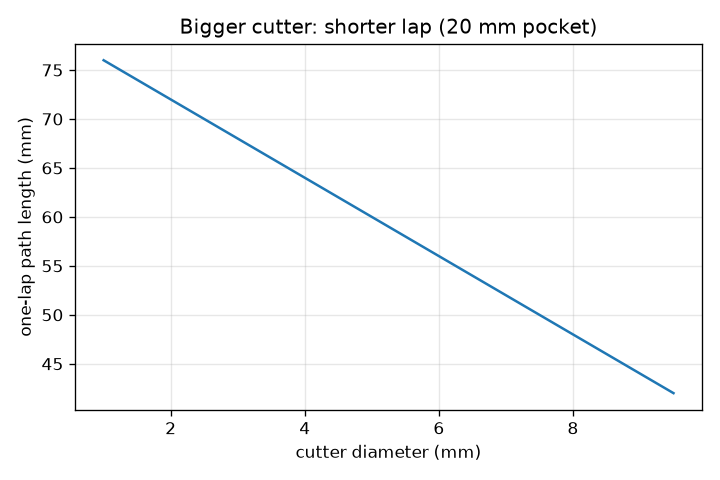
\includegraphics[width=0.85\linewidth]{figures/s01_lap_length_vs_diameter.png}\\\small One-lap path length against cutter diameter for a 20 mm pocket.\end{center}

\subsection*{E. Worked example}
A 20 mm square pocket is cut with a 4 mm cutter at 120 mm/min. Find the centre path, its length, the time for one lap and the island that is left.
\begin{enumerate}[nosep]
\item Radius r = 4 / 2 = 2 mm. The centre path is the square from 2 mm to 18 mm in x and y, with side 16 mm.
\item Length L = 4 * 16 = 64 mm.
\item Time = 64 / 120 min = 0.533 min = 32.0 s.
\item Island side = 20 - 4 * 2 = 12 mm: a 12 mm square in the middle is not touched.
\end{enumerate}
\textbf{Answer.} The cutter centre follows a 16 mm square (64 mm long); one lap takes 32.0 s and leaves a 12 mm square island.

\subsection*{F. Questions}
\begin{enumerate}[nosep]
\item \textbf{Conceptual.} Why does the cutter centre have to follow a path one radius inside the wall, and why does one lap of a big pocket leave an island?
\item \textbf{Numerical.} A 30 mm square pocket is cut with a 6 mm cutter at 150 mm/min. Find the path length, the time for one lap and the island side.
\item \textbf{Graph and simulation interpretation.} In the time graph the curve falls as the feed rises. If the feed is halved from 120 to 60 mm/min for the 64 mm path, what happens to the time? What does the curve shape say?
\item \textbf{Design and optimisation challenge.} Design: choose a cutter diameter and a feed to clear a 20 mm pocket in one lap, with no island, in under 20 s. Is there a limit on the feed?
\end{enumerate}

\section{Session 2: G-code, offsets and arcs}

\subsection*{A. Real-world problem}
A CNC controller reads text such as \texttt{G1 X10 Y5 F300}. You will write that text with a tiny Python generator, read it back to check the geometry, and use it to plan a pocket: a 40 x 30 mm pocket, 5 mm deep, with a 6 mm cutter taking at most 2 mm depth per pass. How many passes and lines are needed, and how long will it take? Educational toolpath geometry only: real machining needs trained operators, machine-specific post-processing and safety checks.

\subsection*{B. Concept and theory}
A G-code line is a list of words, each a letter and a number. G0 is a rapid move (not cutting) and G1 a straight cutting move; X, Y, Z are target coordinates in mm (G21 mm, G90 absolute); F is the feed in mm/min. G2 is a clockwise and G3 a counter-clockwise circular arc to (X, Y); I and J are the offsets from the START point to the arc centre, so the centre is (x0 + I, y0 + J). A valid arc has the same radius sqrt(I\textasciicircum{}2 + J\textasciicircum{}2) at the start and at the end, and its length is the radius times the swept angle in radians. Words are modal: a missing coordinate, the G word and F keep their last values. The toolpath is an offset curve of the part outline: for a pocket the cutter centre follows the outline moved inwards by r (a w x h rectangle becomes (w - 2r) x (h - 2r)); for a profile around a part it follows the outline moved outwards by r, and the rectangle's corners become arcs of radius r. A pocket is cleared with zigzag lines along x spaced by at most the stepover s, in layers of at most the depth of cut. The time is the cutting length divided by the feed, plus the plunge.

\begin{itemize}[nosep]
\item X, Y, Z: target coordinates (absolute) (mm)
\item F: feed rate (mm/min)
\item I, J: arc centre minus arc start (mm)
\item r: cutter radius (D/2) (mm)
\item D: cutter diameter (mm)
\item s: stepover between lines (mm)
\item n: number of zigzag lines (no unit)
\item N: number of depth layers (no unit)
\item doc: depth of cut per layer (mm)
\item T: machining time (s)
\end{itemize}

\begin{equation*}
T=\frac{L}{F}\cdot 60\ \text{s}\quad(L\ \text{in mm},\ F\ \text{in mm/min})
\end{equation*}

\begin{equation*}
\text{centre}=(x_0+I,\ y_0+J),\qquad R=\sqrt{I^2+J^2},\qquad L_{\text{arc}}=R\,\theta
\end{equation*}

\begin{equation*}
\text{pocket path: }(w-D)\times(h-D),\qquad \text{profile path: }(w+D)\times(h+D)\ \text{with corner arcs of radius }r
\end{equation*}

\begin{equation*}
n=\left\lceil\frac{h-D}{s}\right\rceil+1,\qquad N=\left\lceil\frac{\text{depth}}{doc}\right\rceil,\qquad L_{\text{layer}}=n\,(w-D)+(h-D)
\end{equation*}

\begin{equation*}
T=\frac{N\,L_{\text{layer}}}{F}\cdot 60+\frac{\text{depth}+0.5}{F_{\text{plunge}}}\cdot 60
\end{equation*}

\begin{center}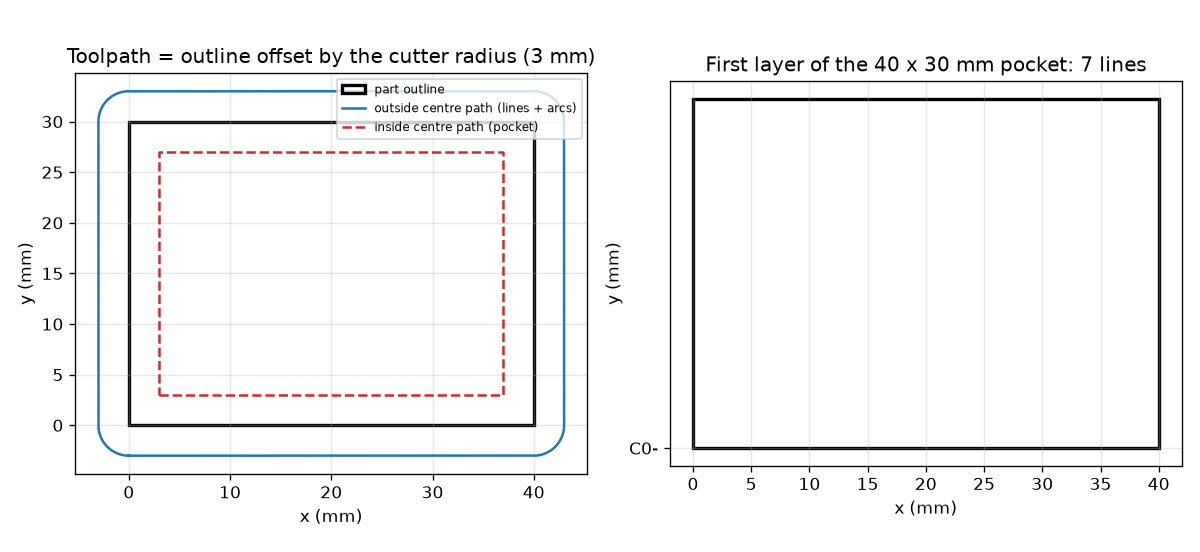
\includegraphics[width=0.85\linewidth]{figures/s02_offsets_and_pocket.png}\\\small Offsets of a 40 x 30 mm outline by 3 mm (pocket inside, profile outside with corner arcs) and the first layer of the pocket.\end{center}

\subsection*{E. Worked example}
Design: clear a 40 x 30 mm pocket, 5 mm deep, with a 6 mm cutter and a 2 mm depth of cut per pass at 300 mm/min. Choose the stepover and the number of passes and estimate the time.
\begin{enumerate}[nosep]
\item The centre must cover (40 - 6) x (30 - 6) = 34 x 24 mm, so lines run 34 mm long and cover a 24 mm span.
\item Choose the stepover at most 75 percent of the diameter: 4.5 mm. Lines n = ceil(24 / 4.5) + 1 = 7, spaced evenly at 24 / 6 = 4.0 mm.
\item Layers N = ceil(5 / 2) = 3, each 5 / 3 = 1.667 mm deep.
\item One layer: 7 * 34 + 24 = 262 mm; three layers: 786 mm.
\item Cutting time = 786 / 300 min = 2.62 min = 157.2 s. Plunge: 5.5 mm / 100 mm/min = 3.3 s. Total 160.5 s.
\item Parsing our own G-code gives the same 160.5 s for cutting and plunging; adding rapids at 3000 mm/min gives 162.6 s.
\end{enumerate}
\textbf{Answer.} Stepover 4.5 mm (7 lines, 4 mm apart), 3 layers, 786 mm of cutting: about 160.5 s, or 162.6 s with rapids.

\subsection*{F. Questions}
\begin{enumerate}[nosep]
\item \textbf{Conceptual.} The same start (10, 0) and end (0, 10) with I-10 J0 are used for G3 and for G2. Do they give the same arc? Why does the centre not change?
\item \textbf{Numerical.} An arc starts at (20, 0), ends at (0, 20) and is written G3 X0 Y20 I-20 J0. Find the centre, check the end radius and find the arc length.
\item \textbf{Graph and simulation interpretation.} On the time-against-stepover graph, the time is 282.9 s at a stepover of 2 mm and 119.7 s at 6 mm. Why does the curve fall quickly at first and then flatten? Why can the stepover not exceed 6 mm?
\item \textbf{Design and optimisation challenge.} Design: repeat the plan with an 8 mm cutter (stepover at most 75 percent of D, depth of cut 2 mm, 300 mm/min, plunge 100 mm/min). How many lines, how much cutting length and what time? Is it faster than the 6 mm cutter, and what is the catch?
\end{enumerate}

\section{Session 3: Pocketing strategies and a simulation that checks them}

\subsection*{A. Real-world problem}
A toolpath that looks right can still leave material behind, cut too much, or take twice as long as it should. We cut a simulated block on a grid of heights (a height-map), subtract the cutter footprint along the path, and compare the removed volume and the leftover ridges with formulas. At the end we generate G-code for a pocket with a round boss and check its removed volume. Educational toolpath geometry only: real machining needs trained operators, machine-specific post-processing and safety checks; the feeds and speeds here are teaching numbers.

\subsection*{B. Concept and theory}
The height-map stores the height of the material top in each grid cell (0 = original top). A flat-end cutter at (x, y) with tip height z sets every cell within its radius to at most z; a ball-end cutter of radius r leaves height z + r - sqrt(r\textasciicircum{}2 - rho\textasciicircum{}2) at distance rho from its axis. Raster pocketing uses parallel lines; contour-parallel pocketing offsets the outline inwards by r, r + s, r + 2s, and so on. Neighbouring ball-end passes s apart leave a ridge midway of height h = r - sqrt(r\textasciicircum{}2 - (s/2)\textasciicircum{}2); inversely s = 2 sqrt(2 r h - h\textasciicircum{}2). The material removal rate is MRR = a\_e a\_p F (radial width, axial depth, feed) and the chip load is f\_z = F / (N z) for N rev/min and z teeth. A round flat cutter cannot reach into a sharp inside corner: each of the four corners keeps r\textasciicircum{}2 (1 - pi/4) of area, so the pocket keeps 4 r\textasciicircum{}2 (1 - pi/4). A stepover larger than the cutter diameter D leaves strips of width s - D. An offset in the wrong direction makes the cutter cut outside the pocket. A slot narrower than the cutter cannot be cut, and the planner must report that.

\begin{itemize}[nosep]
\item r: cutter radius (mm)
\item s: stepover between passes (mm)
\item h: ridge (scallop) height (mm)
\item a\_e: radial width of cut (mm)
\item a\_p: axial depth of cut (mm)
\item F: feed rate (mm/min)
\item N: spindle speed (rev/min)
\item z: number of cutting teeth (no unit)
\item f\_z: chip load, feed per tooth (mm)
\item MRR: material removal rate (mm\textasciicircum{}3/min)
\end{itemize}

\begin{equation*}
h=r-\sqrt{r^{2}-\left(\frac s2\right)^{2}},\qquad s=2\sqrt{2rh-h^{2}}
\end{equation*}

\begin{equation*}
\mathrm{MRR}=a_e\,a_p\,F,\qquad f_z=\frac{F}{N\,z}
\end{equation*}

\begin{equation*}
A_{\text{corners}}=4\,r^{2}\left(1-\frac{\pi}{4}\right)
\end{equation*}

\begin{equation*}
A_{\text{gouge}}=(w+4r)(h+4r)-(4-\pi)r^{2}-wh\quad(\text{centre path offset outwards by } r)
\end{equation*}

\begin{equation*}
V=\left(wh-\pi R_b^{2}-4r^{2}\left(1-\tfrac{\pi}{4}\right)\right)\,\text{depth}\quad(\text{pocket with a boss of radius } R_b)
\end{equation*}

\begin{center}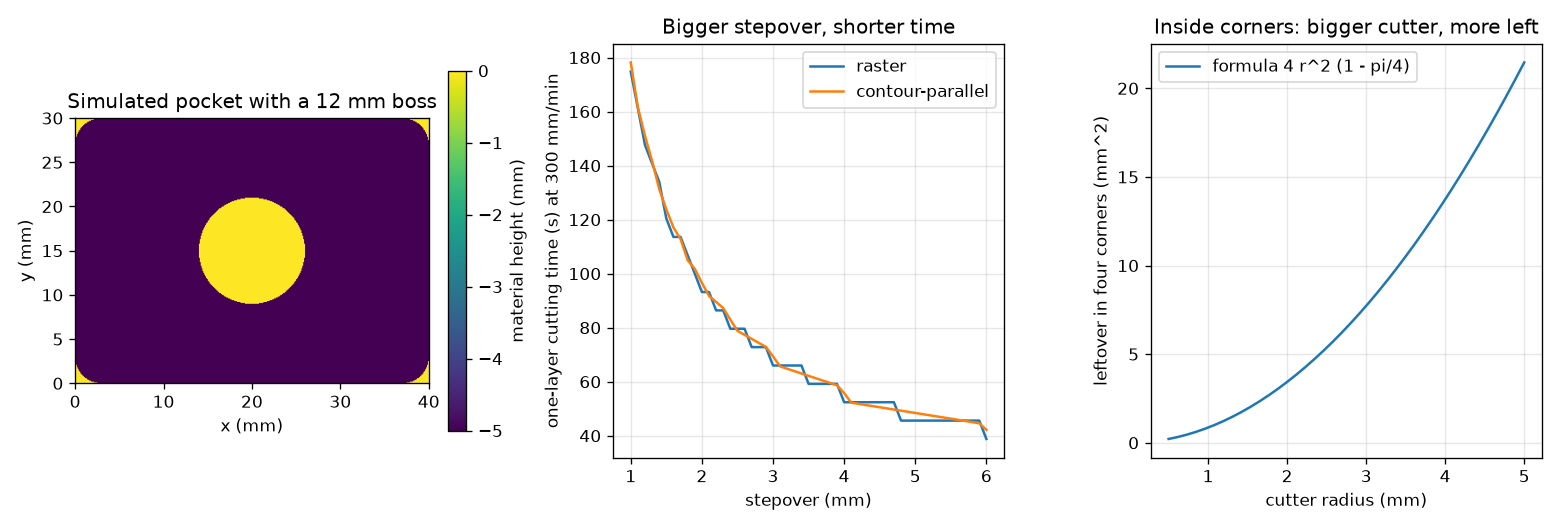
\includegraphics[width=0.85\linewidth]{figures/s03_boss_and_tradeoffs.png}\\\small Simulated boss pocket, one-layer time against stepover for two strategies, and the corner leftover against the cutter radius.\end{center}

\subsection*{E. Worked example}
A ball-end cutter of radius 3 mm makes parallel passes 2 mm apart. Find the ridge height, then the largest stepover that keeps the ridge at 0.05 mm or less, and check by simulation.
\begin{enumerate}[nosep]
\item h = 3 - sqrt(3\textasciicircum{}2 - 1\textasciicircum{}2) = 3 - sqrt(8) = 3 - 2.828 = 0.1716 mm.
\item For h = 0.05 mm: s = 2 sqrt(2 * 3 * 0.05 - 0.05\textasciicircum{}2) = 2 sqrt(0.2975) = 2 * 0.5454 = 1.0909 mm.
\item Use s = 1.0 mm (a convenient value below the limit): h = 3 - sqrt(9 - 0.25) = 0.0420 mm. With 1.1 mm the ridge is 0.0508 mm, just too high.
\item The height-map simulation of 5 passes at 2 mm gives 0.1716 mm (and 0.0420 mm at 1 mm), equal to the formula to better than 0.002 mm.
\end{enumerate}
\textbf{Answer.} Ridge 0.1716 mm at 2 mm stepover; to stay at 0.05 mm or less use at most 1.0909 mm, for example 1.0 mm (ridge 0.0420 mm). The simulation agrees.

\subsection*{F. Questions}
\begin{enumerate}[nosep]
\item \textbf{Conceptual.} Why does a bigger stepover finish a job faster but leave more material behind? Why does the contour-parallel path with stepover equal to the diameter still leave cusps in the corners?
\item \textbf{Numerical.} A cutter has 2 teeth, runs at 8000 rev/min and feeds at 480 mm/min. Find the chip load. Then find the MRR for a\_e = 3 mm, a\_p = 1.5 mm and F = 400 mm/min.
\item \textbf{Graph and simulation interpretation.} In the corner-leftover graph, read the leftover area for a cutter radius of 3 mm and of 5 mm. What happens when the radius doubles, and what does that say about choosing a cutter?
\item \textbf{Design and optimisation challenge.} Design: a ball-end cutter of radius 4 mm must finish a 40 x 30 mm face with a ridge of at most 0.02 mm at 600 mm/min. Choose a stepover (rounded down to 0.01 mm), count the lines and estimate the time. Lines run along the 40 mm side, plus 30 mm of side-steps in total.
\end{enumerate}

\section{Session 4: Offset any convex polygon}

\subsection*{A. Real-world problem}
Sessions 2 and 3 could offset only a rectangle: shrink each side by the cutter radius. A hexagonal pocket (a nut seat, a bolt-head recess) has six sides at 120 degrees, and the rectangle recipe does not carry over. How far does each corner of the cutter-centre path move? What happens when the offset is larger than the pocket allows? Can the same idea give a complete pocket path? Today we offset a convex polygon edge by edge, find the distance at which the offset collapses, repair the case where one edge disappears before the others, and cut a hexagonal pocket whose G-code we read back and simulate. Educational toolpath geometry only.

\subsection*{B. Concept and theory}
A convex polygon is listed counter-clockwise, so that its inside is on the left of every edge, and every turn is to the left. At a corner the interior angle theta is the angle between the two edges, measured inside. The \textbf{inward offset} by d moves every edge d along its inward normal; two neighbouring shifted lines meet in a new corner. That corner lies on the bisector of the old one, d / sin(theta / 2) away from it. Each edge keeps its direction and changes its length to L' = L - d (cot(theta\_a / 2) + cot(theta\_b / 2)), and while no edge has vanished the area is A(d) = A - P d + d\textasciicircum{}2 sum of cot(theta\_i / 2), with P the perimeter. For the hexagon of side 20 mm and d = 3 mm the corner shift is 3.464 mm, the new side is 16.536 mm and the area is 710.41 mm\textasciicircum{}2.

The recipe breaks when an edge reaches length zero before the others: the two neighbouring shifted lines then cross behind each other and the result has a reversed edge. The correct offset is the \textbf{intersection of the shifted half-planes}: the part of the polygon that is at least d from every edge line. We compute it by clipping the polygon against one shifted line after another. An edge that vanishes simply drops out; when nothing is left the offset has \textbf{collapsed}. The collapse distance is the radius of the largest circle inside the polygon; for a regular polygon it is the apothem a / (2 tan(pi / n)), 17.32 mm for the hexagon of side 20 mm.

A cutter of diameter D (radius r) keeps its centre at least r from every wall, so its centre path is the polygon offset by r. To clear the pocket, cut rings at the offsets r, r + s, ... up to the collapse distance rho, with the stepover s at most D: n = ceil((rho - r) / s) + 1 rings, spaced evenly so that the last ring sits exactly at the collapse. The rings are cut from the wall inwards and joined by short straight links inside the area already cleared, so the cutter plunges once per layer. A round cutter cannot reach into a sharp corner: each corner of interior angle theta keeps r\textasciicircum{}2 (cot(theta / 2) - (pi - theta) / 2) of leftover area.

\begin{itemize}[nosep]
\item d: inward offset distance (mm)
\item theta: interior angle at a corner (radians)
\item L, L': edge length before and after the offset (mm)
\item A, P: polygon area and perimeter (mm\textasciicircum{}2 and mm)
\item rho: collapse distance (inscribed-circle radius) (mm)
\item r, D: cutter radius and diameter (mm)
\item s: stepover between rings (mm)
\end{itemize}

\begin{equation*}
\Delta_{\text{corner}}=\frac{d}{\sin(\theta/2)},\qquad L'=L-d\left(\cot\frac{\theta_a}{2}+\cot\frac{\theta_b}{2}\right),\qquad A(d)=A-Pd+d^{2}\sum_i\cot\frac{\theta_i}{2}
\end{equation*}

\begin{equation*}
\rho_{\text{regular}}=\frac{a}{2\tan(\pi/n)},\qquad n_{\text{rings}}=\left\lceil\frac{\rho-r}{s}\right\rceil+1,\qquad \text{leftover per corner}=r^{2}\left(\cot\frac{\theta}{2}-\frac{\pi-\theta}{2}\right)
\end{equation*}

\begin{center}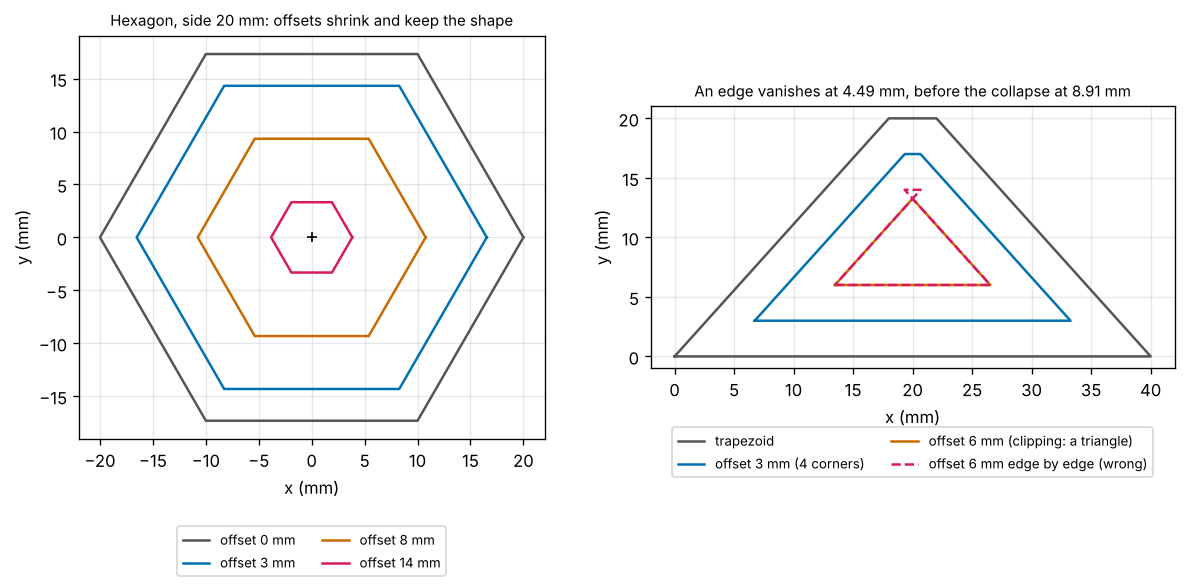
\includegraphics[width=0.95\linewidth]{figures/s04_offsets_and_vanishing_edge.png}\\\small Hexagon offsets, and a trapezoid whose top edge vanishes before the collapse.\end{center}

\begin{center}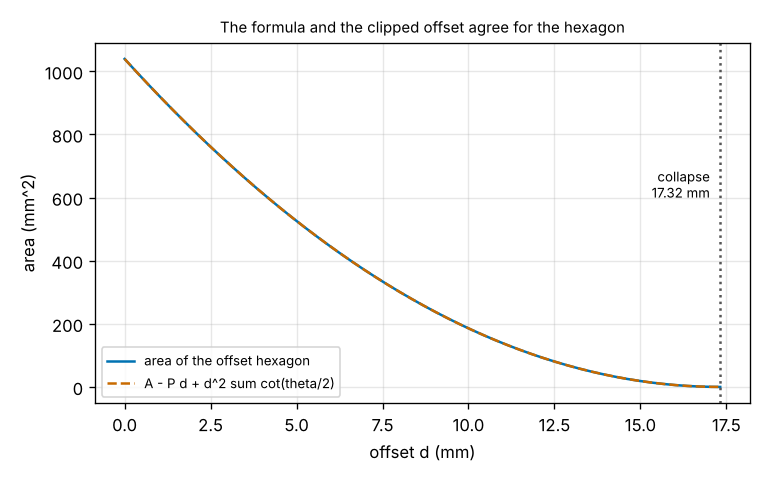
\includegraphics[width=0.6\linewidth]{figures/s04_area_vs_offset.png}\\\small Area of the offset hexagon: clipping and formula.\end{center}

\begin{center}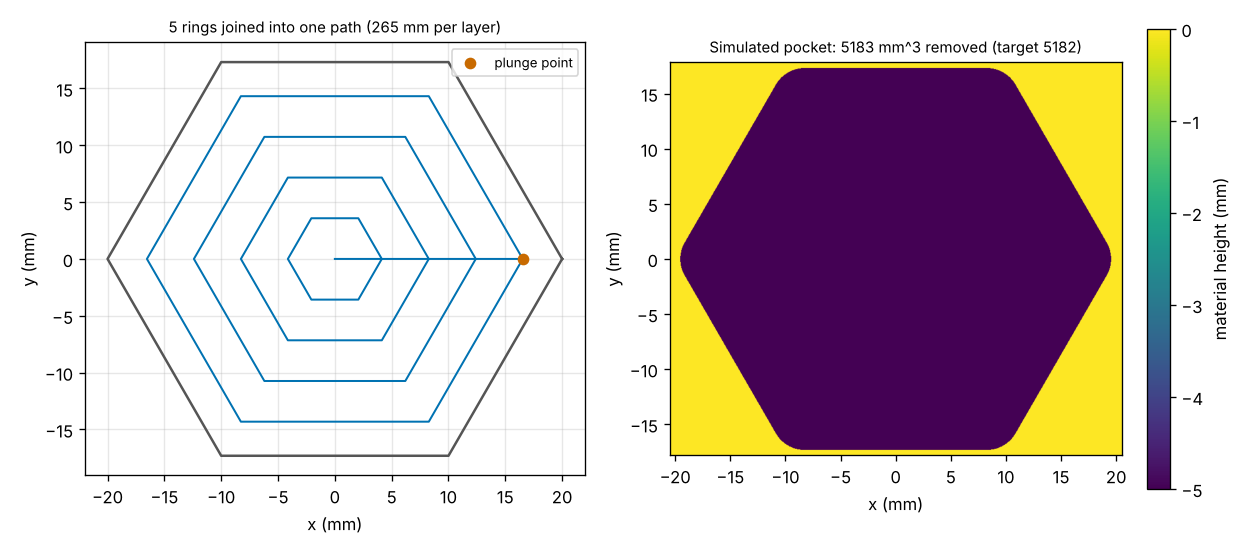
\includegraphics[width=0.95\linewidth]{figures/s04_hexagon_pocket.png}\\\small The ring path of the hexagon pocket and the simulated height-map.\end{center}

\subsection*{E. Worked example}
A regular hexagon has side 20 mm. Offset it inwards by 3 mm. Find the corner shift, the new side length, the new area and the distance at which the offset collapses.
\begin{enumerate}[nosep]
\item The interior angle is 120 degrees, so theta / 2 = 60 degrees.
\item The corner shift is d / sin 60 = 3 / 0.8660 = 3.4641 mm.
\item The new side is 20 - 3 (cot 60 + cot 60) = 20 - 3 x 1.1547 = 16.5359 mm.
\item The new area is (3 sqrt 3 / 2) x 16.5359\textasciicircum{}2 = 710.41 mm\textasciicircum{}2; the formula gives 1039.23 - 120 x 3 + 9 x 6 x 0.5774 = 710.41 mm\textasciicircum{}2.
\item The offset collapses at the apothem 20 / (2 tan 30) = 17.3205 mm; for a larger d nothing is left.
\end{enumerate}
\textbf{Answer.} The corners move 3.464 mm, the new side is 16.536 mm, the new area is 710.41 mm\textasciicircum{}2 and the collapse is at 17.32 mm.

\subsection*{F. Questions}
\begin{enumerate}[nosep]
\item \textbf{Conceptual.} Why does a corner of the offset hexagon move by more than the offset distance, and why does the edge-by-edge recipe work for the hexagon but fail for the trapezoid of Figure 1?
\item \textbf{Numerical.} A regular octagon has side 10 mm. Offset it inwards by 2 mm. Find the interior angle, how far the corners move, the new side length, the area of the offset octagon and the distance at which it collapses.
\item \textbf{Graph and simulation interpretation.} In the right panel of Figure 1 (and in the app, with the trapezoid and d = 6 mm) the dashed outline has a small hook at the top. What went wrong, and how far from the right-hand wall are the two hook corners? What would a cutter of radius 6 mm do if it followed that outline?
\item \textbf{Design and optimisation challenge.} Design: a hexagonal recess for a nut, 24 mm across the flats, 5 mm deep, to be cut with a 6 mm cutter. Plan it: the side length, the number of rings for a stepover of 40 percent of the diameter, the layers, the cutting time (feed 300 mm/min, plunge 100 mm/min), and what the nut will see in the corners.
\end{enumerate}

\section{Session 5: A pocket with a boss, cut without lifting}

\subsection*{A. Real-world problem}
The Session 3 program for the 40 x 30 mm pocket with a 12 mm boss cuts it in rows. Every row that meets the boss is cut in two pieces, and every piece is a lift, a rapid move and a plunge: 14 plunges per layer and 42 in all, and 315.5 s of cutting. A contour-parallel path follows the walls and the boss at a steady distance and can be one unbroken cut. The hard part is the join: as the rings move inward they touch the ring round the boss, split into two crescents at the narrow neck, and finally shrink to four points. Today we build that path from the clearance field (how far the cutter centre is from the nearest wall or the boss), cut it with straight moves and arcs, and check the time, the volume and the coverage. Educational toolpath geometry only.

\subsection*{B. Concept and theory}
The cutter centre may stand at a point only if the whole cutter fits: at least r from every wall and at least r\_b + r from the boss centre. The \textbf{clearance} of a point is its distance to the nearest wall or to the boss surface, and the centre may stand where the clearance is at least r. The set of points with a given clearance l is the \textbf{ring} at l, a closed outline of the cutter-centre path: the boundary of the rectangle shrunk by l, minus a disc of radius r\_b + l round the boss centre. It consists of \textbf{line pieces} (the sides of the shrunk rectangle that are outside the disc) and \textbf{arc pieces} (the circle where it is inside the rectangle). The first ring is at l = r, where the cutter touches the walls. Rings farther in have a larger l, up to the \textbf{largest clearance} rho, the clearance of the point deepest inside the pocket; the 40 x 30 mm pocket with the 12 mm boss has rho = 7.9546 mm.

The rings change shape as l grows. At first the ring is one rectangle with the boss circle as a hole. When the passage between the boss and a wall closes, at l = gap / 2 (4.5 mm at the top and bottom), the ring falls into pieces: a left and a right crescent. Further in, the crescents shrink to the four points where two walls and the boss are equally far. Every piece of a ring lies inside exactly one piece of the previous ring, so the pieces form a \textbf{tree}; a depth-first walk of the tree visits every piece, and between pieces the cutter moves along a \textbf{link}: a straight line if that stays outside the circle of radius r\_b + r round the boss centre, otherwise a tangent line to that circle, an arc along it and a tangent line off it. All of this is in the space where the cutter centre may stand, which is cut anyway, so the cutter never has to lift inside a layer.

The rings are placed at l = r, r + s, r + 2 s, ... (stepover s, at most D), and a last ring at rho is added if the cutter, which reaches r past the last ring, would not reach it. That is not enough where a ring splits: the point in the middle of a closing passage is far from the ring on either side. So the planner checks the coverage on a grid of 0.25 mm and adds a ring just below the worst uncovered point, until every point of the pocket is within r of the path (except the rounded leftovers in the four corners). The path is written as G1 for the lines and G2 (clockwise) or G3 for the arcs.

\begin{itemize}[nosep]
\item w, h: pocket width and height (mm)
\item c, r\_b: boss centre and radius (mm)
\item r, D: cutter radius and diameter (mm)
\item s: stepover between rings (mm)
\item l (ell): clearance of a ring (mm)
\item rho: largest clearance (mm)
\item R: radius of the link circle, r\_b + r (mm)
\end{itemize}

\begin{equation*}
\varphi(x,y)=\min\Big(x,\; w-x,\; y,\; h-y,\; \lVert (x,y)-c\rVert - r_b\Big),\qquad \text{ring at clearance } \ell:\ \varphi=\ell,\qquad \text{centre may stand where } \varphi\ge r
\end{equation*}

\begin{equation*}
\ell_{\text{neck}}=\tfrac12\,\text{gap},\qquad \rho_{\max}=(c_x+c_y+r_b)-\sqrt{(c_x+c_y+r_b)^2-(c_x^2+c_y^2-r_b^2)},\qquad \text{link}=\sqrt{d_p^2-R^2}+\sqrt{d_q^2-R^2}+R\,\Delta\alpha
\end{equation*}

\begin{center}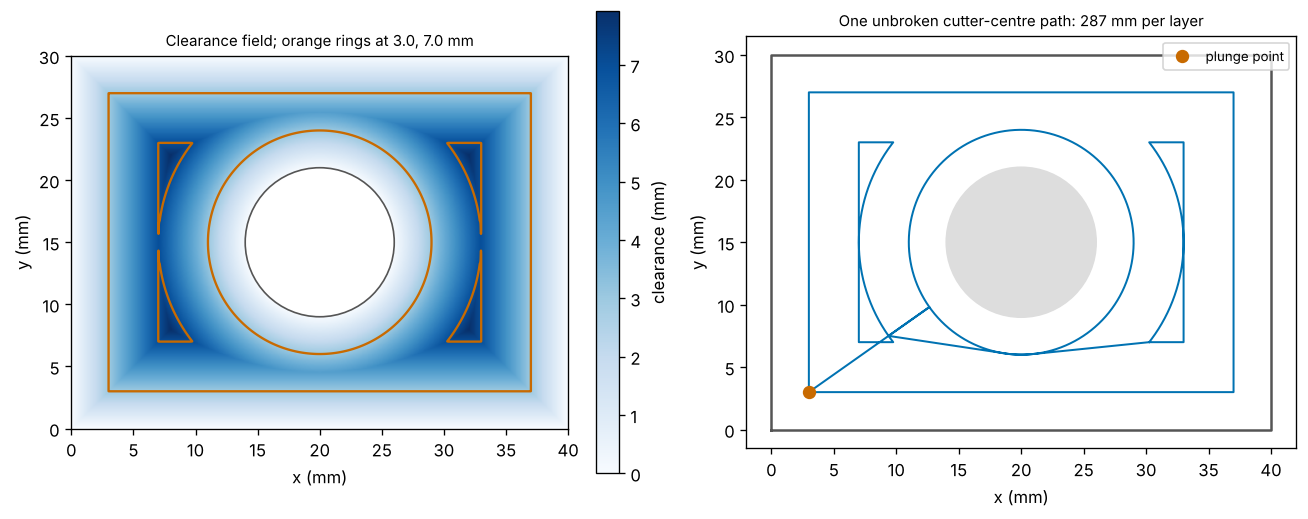
\includegraphics[width=0.95\linewidth]{figures/s05_clearance_and_path.png}\\\small The clearance field with the rings at 3 and 7 mm, and the one-layer path.\end{center}

\begin{center}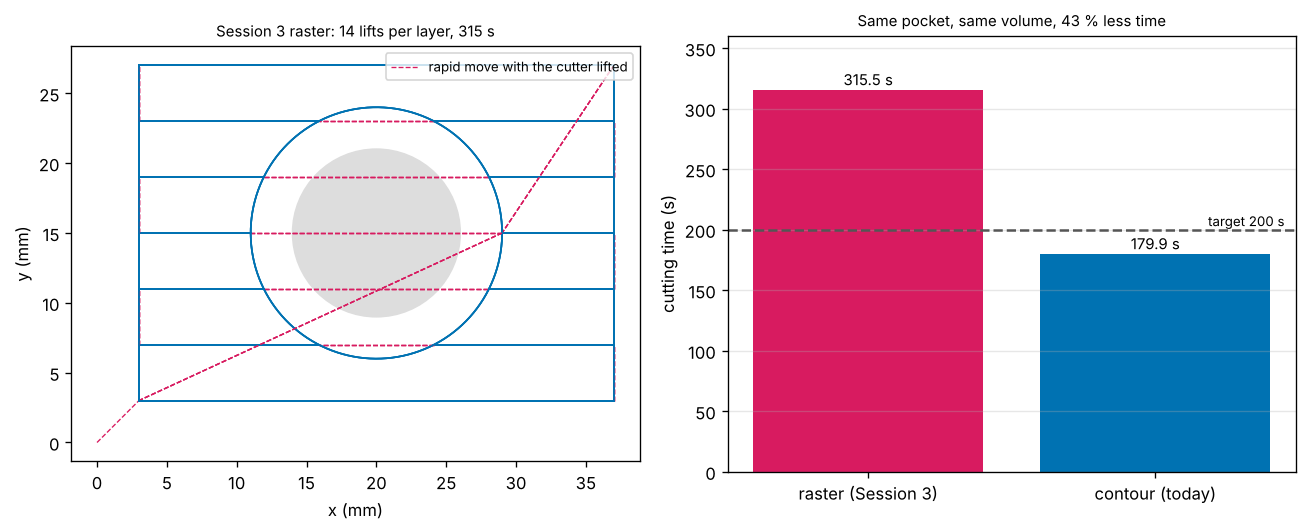
\includegraphics[width=0.95\linewidth]{figures/s05_raster_vs_contour.png}\\\small The raster program with its lifts, and the cutting time of both programs.\end{center}

\begin{center}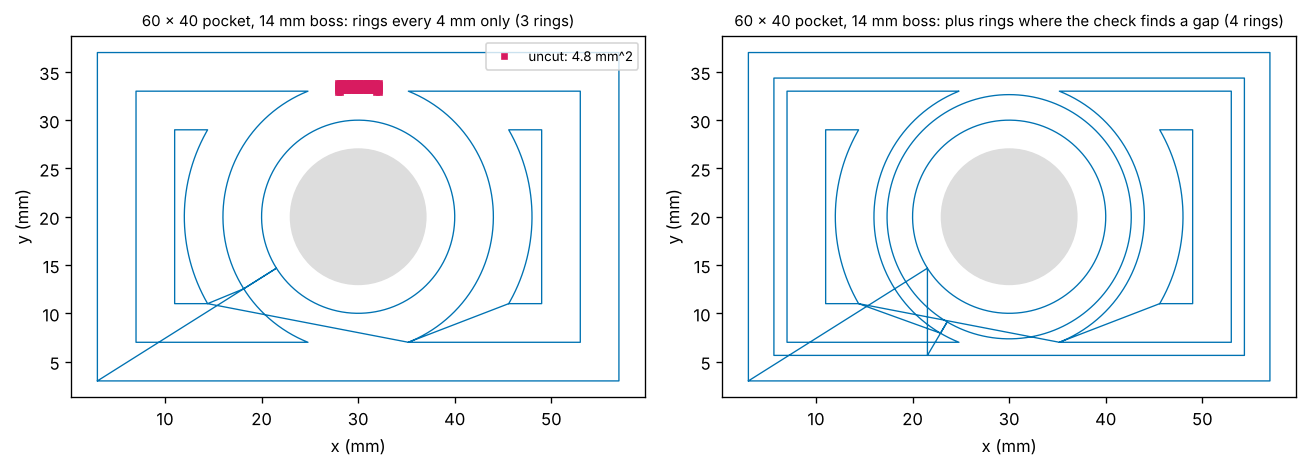
\includegraphics[width=0.95\linewidth]{figures/s05_gap_at_split.png}\\\small Rings every 4 mm leave a block where a ring splits; the coverage check adds a ring.\end{center}

\subsection*{E. Worked example}
The 40 x 30 mm pocket has a round boss of diameter 12 mm at (20, 15). The cutter is 6 mm, the stepover 4 mm. Find the clearance at which the passage above the boss closes, the largest clearance, and the ring schedule.
\begin{enumerate}[nosep]
\item The boss radius is 6 mm and its top is at y = 21 mm; the top wall is at y = 30 mm, so the gap is 9 mm.
\item The passage closes when the two rings use it up: 2 l = 9 mm, so l = 4.5 mm.
\item The deepest points are the corners: (20 - l)\textasciicircum{}2 + (15 - l)\textasciicircum{}2 = (6 + l)\textasciicircum{}2, so l\textasciicircum{}2 - 82 l + 589 = 0 and l = 41 - sqrt(1092) = 7.9546 mm.
\item The rings are at r = 3 mm and r + s = 7 mm. The next would be 11 mm, beyond 7.9546 mm. The cutter reaches 3 mm past the ring at 7 mm, which is 10 mm, beyond 7.9546 mm, so no last ring is needed.
\end{enumerate}
\textbf{Answer.} The passage closes at 4.5 mm, the largest clearance is 7.9546 mm and the rings are at 3 mm and 7 mm.

\subsection*{F. Questions}
\begin{enumerate}[nosep]
\item \textbf{Conceptual.} In the 40 x 30 mm pocket with the 12 mm boss and a 6 mm cutter, the ring at clearance 4.4 mm is one closed outline with the boss circle as a hole, but the ring at 4.6 mm is in two pieces. Why does the split happen between those values, and why do the rings end in four points at 7.95 mm?
\item \textbf{Numerical.} A 50 x 30 mm pocket has a round boss of diameter 10 mm at its centre (25, 15) and is cut with a 6 mm cutter and a stepover of 4 mm. Find the clearance at which the passage above the boss closes, the largest clearance, the length of the first ring, and the clearance of every ring.
\item \textbf{Graph and simulation interpretation.} In the left panel of Figure 3 (a 60 x 40 mm pocket with a 14 mm boss) the rings are 4 mm apart, yet there is a pink block of uncut material above the boss. How wide and how high is it, and why do rings that are at most the stepover apart leave it? What does the repair in the right panel cost?
\item \textbf{Design and optimisation challenge.} Design: cut the 50 x 30 mm pocket with the 10 mm boss of question B, 5 mm deep, with a 6 mm cutter, depth of cut 2 mm, stepover 4 mm, feed 300 mm/min and plunge 100 mm/min. Plan it with the contour planner and compare it with the Session 3 raster program: layers, plunges, cutting time and volume.
\end{enumerate}

\section{Real-world mini-project}
\textbf{Generate G-code for a pocket with a boss and check it.} A 40 x 30 mm pocket, 5 mm deep, has a round boss of diameter 12 mm in the middle at (20, 15) that must stay. Use a 6 mm flat cutter, 2 mm depth of cut per layer, stepover 4 mm, feed 300 mm/min, plunge 100 mm/min and rapids at 3000 mm/min. Use \texttt{boss\_pocket\_gcode} from Session 3, parse the text back with \texttt{read\_moves}, simulate it on a height-map with \texttt{simulate\_moves}, and compare the removed volume with the analytic volume.

\textbf{Offset any convex polygon and cut a hexagonal pocket.} Use the lesson's \texttt{offset\_polygon}, \texttt{collapse\_distance}, \texttt{ring\_offsets}, \texttt{pocket\_path} and \texttt{pocket\_gcode}. The roadmap target is that every corner of the offset hexagon (side 20 mm, offset 3 mm) lies 3 mm from its two neighbouring edges within 1e-6 mm (the shipped Sessions 2 and 3 code offsets only rectangles). \textbf{Deliverable:} A script that returns the inward offset of any convex polygon (or None when it has collapsed), checks every corner of the offset hexagon against its two neighbouring edges, prints the collapse distance and the first distance at which an edge vanishes, writes the G-code of a hexagonal pocket (side 20 mm, 5 mm deep, 6 mm cutter, stepover 4 mm, depth of cut 2 mm), reads it back, and compares the simulated volume with the analytic one. It saves the graph of the offsets. \textbf{Success looks like:} The six corners of the offset hexagon are 3 mm from their two neighbouring edges to within 5e-15 mm (needed: 1e-6 mm) and farther from the other four. The collapse is at 17.3205 mm, the apothem. The trapezoid loses its top edge at 4.49 mm and collapses at 8.91 mm; at 6 mm the edge-by-edge outline has a reversed edge of -1.34 mm and an area of 46.845 mm\textasciicircum{}2, against 47.347 mm\textasciicircum{}2 for the triangle from clipping. The pocket has 5 rings at offsets 3.0, 6.58, 10.16, 13.74 and 17.32 mm, a path of 264.6 mm per layer, 3 layers with 3 plunges, a cutting time of 166.5 s (167.9 s with rapids), a simulated volume of 5182.7 mm\textasciicircum{}3 against 5181.6 mm\textasciicircum{}3 analytic (+0.02 percent) and 2.90 mm\textasciicircum{}2 of corner leftover.

\textbf{Contour-parallel pocket with a boss.} The roadmap pocket: 40 x 30 mm, 5 mm deep, a boss of diameter 12 mm at (20, 15), a 6 mm cutter, stepover 4 mm, depth of cut 2 mm, feed 300 mm/min, plunge 100 mm/min. Use the lesson's \texttt{plan\_pocket}, \texttt{contour\_gcode} and \texttt{simulate\_contour}, and the Session 3 \texttt{boss\_pocket\_gcode} as the baseline. The roadmap target is a cutting time (G1, G2, G3 and plunge moves) under 200 s and a simulated volume within 0.5 percent of 5395.9 mm\textasciicircum{}3, with no retract inside a layer (the shipped program needs 315.5 s). \textbf{Deliverable:} A script that plans the path, writes the G-code, reads it back, prints the cutting time, the number of plunges and lifts, and the simulated and analytic volumes with their difference, compares them with the Session 3 raster program, and saves the pictures. \textbf{Success looks like:} The largest clearance is 7.9546 mm and the rings are at 3 mm and 7 mm. One layer is 286.9 mm and the cutting time is 179.9 s (181.5 s with rapids) against 315.5 s for the raster program, with 3 plunges (one per layer) against 42. The simulated volume is 5396.2 mm\textasciicircum{}3 against 5395.9 mm\textasciicircum{}3 analytic (+0.006 percent) and nothing is cut inside the boss. The cutter centre never gets closer than 3.000 mm to a wall or 9.000 mm to the boss centre, and the coverage check finds no uncut point. For the 60 x 40 mm pocket with a 14 mm boss it finds a 4.75 mm\textasciicircum{}2 block, adds a ring at 5.64 mm and the volume is again within 0.006 percent.

\section{The path ahead}
\begin{enumerate}[nosep]
\item \textbf{Session 6: Rest machining of the corners.} A second pass with a 2 mm cutter that follows the corner leftover left by the 6 mm cutter.
\item \textbf{Session 7: 3D ball-end finishing.} Parallel finishing passes over a hemisphere of radius 15 mm with a ball cutter of radius 3 mm, simulated on a 3D height-map.
\item \textbf{Session 8: Post-processor dialects.} A writer that outputs arcs with I, J and with the R word, and a parser that reads both.
\end{enumerate}

\section{Answers and hints}

\subsection*{Session 1}
\begin{enumerate}[nosep]
\item \textbf{Conceptual.} Hint: Where is the cutter edge relative to its centre? How far from the path does the cutter reach? Solution: The cutter edge is one radius from its centre, so for the edge to touch the wall the centre must be one radius from the wall. The cutter only removes material within one radius of its centre, so a single lap clears a strip of width 2r = d along the wall; if the pocket is wider than 4r, the middle is out of reach and remains as an island.
\item \textbf{Numerical.} Hint: L = 4 (side - d); t = L / F * 60; island = side - 2d. Solution: L = 4 * (30 - 6) = 96 mm. Time = 96 / 150 * 60 = 38.4 s. Island side = 30 - 12 = 18 mm. Sanity check: a bit more than 3 times the pocket side for the path, and a slow feed (150 mm/min is 2.5 mm per second) gives tens of seconds.
\item \textbf{Graph and simulation interpretation.} Hint: t = L / F * 60. Solution: The time doubles from 32 s to 64 s. The curve is a hyperbola (time inversely proportional to feed): steep at low feeds, flat at high feeds, so the first increases in feed save the most time.
\item \textbf{Design and optimisation challenge.} Hint: No island needs side \textless{}= 2d. Then t = 4 (side - d) / F * 60 \textless{} 20. Solution: Side \textless{}= 2d needs d \textgreater{}= 10 mm; take d = 10 mm. The path is 4 * (20 - 10) = 40 mm. Time under 20 s needs F above 40 / 20 * 60 = 120 mm/min (exactly 20.0 s at 120); choose 200 mm/min for 12.0 s. Trade-off: the biggest cutter and a faster feed save time, but real cutters have a maximum feed set by the machine, the material and the cutter, and a 10 mm cutter cannot cut an inside corner sharper than 5 mm radius.
\end{enumerate}

\subsection*{Session 2}
\begin{enumerate}[nosep]
\item \textbf{Conceptual.} Hint: I and J are measured from the start point. Which way round does each word go? Solution: The centre is (10 - 10, 0 + 0) = (0, 0) for both, because it depends only on the start and on I, J. G3 goes counter-clockwise and sweeps 90 degrees (length 15.708 mm); G2 goes clockwise the long way round and sweeps 270 degrees (length 47.124 mm). The endpoints are the same but the arcs are not.
\item \textbf{Numerical.} Hint: centre = start + (I, J); length = R * angle. Solution: Centre = (20 - 20, 0 + 0) = (0, 0). Start radius = 20 mm; end radius = sqrt(0 + 400) = 20 mm, so the arc is valid. Counter-clockwise from 0 to 90 degrees is pi/2 radians, so the length is 20 * pi/2 = 31.416 mm. Units: mm.
\item \textbf{Graph and simulation interpretation.} Hint: Count lines: n = ceil(24 / s) + 1. What does the cutter diameter limit? Solution: Time is mostly the number of lines times the line length, and n falls like 1 / s: halving the stepover roughly doubles the lines, but at large s the lines cannot drop below a few (5 lines at 6 mm). Because n is a whole number the curve also has small steps. The stepover cannot exceed the cutter diameter (6 mm) because then the strip between two lines is wider than the cutter and stays uncut.
\item \textbf{Design and optimisation challenge.} Hint: Span = 30 - 8 = 22 mm; line length = 40 - 8 = 32 mm; stepover at most 6 mm. Solution: n = ceil(22 / 6) + 1 = 5 lines, spaced 5.5 mm. One layer: 5 * 32 + 22 = 182 mm; three layers 546 mm. Time = 546 / 300 * 60 + 3.3 = 109.2 + 3.3 = 112.5 s, faster than 160.5 s. Catch: a bigger cutter rounds the inside corners with a larger radius (4 mm instead of 3 mm), needs more force and may exceed what the machine can hold; Session 3 measures the corner leftover.
\end{enumerate}

\subsection*{Session 3}
\begin{enumerate}[nosep]
\item \textbf{Conceptual.} Hint: Count lines. Then think about where two offset rings meet at a rectangle corner. Solution: A bigger stepover needs fewer lines, so the path is shorter and the time smaller, but the ridge between lines grows (for a ball end) and above the diameter whole strips are left. In contour-parallel paths the rings at a rectangle corner meet at 90 degrees; the round cutter covers a rounded patch, and with spacing equal to the diameter (6 mm for a 3 mm radius) the corner of the next ring is out of reach in the diagonal direction: the simulation clears only 1180.9 mm\textasciicircum{}2 instead of 1192.3 mm\textasciicircum{}2.
\item \textbf{Numerical.} Hint: f\_z = F / (N z); MRR = a\_e a\_p F. Solution: f\_z = 480 / (8000 * 2) = 0.03 mm per tooth. MRR = 3 * 1.5 * 400 = 1800 mm\textasciicircum{}3/min. Units: mm/min divided by rev/min times teeth gives mm per tooth; mm * mm * mm/min gives mm\textasciicircum{}3/min. These are teaching numbers, not recommended cutting conditions.
\item \textbf{Graph and simulation interpretation.} Hint: The curve is 4 r\textasciicircum{}2 (1 - pi/4). Solution: About 7.73 mm\textasciicircum{}2 at 3 mm and 21.46 mm\textasciicircum{}2 at 5 mm. The curve rises with the square of r: doubling the radius quadruples the leftover (3.43 mm\textasciicircum{}2 at r = 2 and 13.73 mm\textasciicircum{}2 at r = 4 also follow the formula). A bigger cutter clears faster but leaves bigger corner fillets, so a smaller cutter is needed to finish the corners (rest machining).
\item \textbf{Design and optimisation challenge.} Hint: Use s = 2 sqrt(2 r h - h\textasciicircum{}2), then n = ceil(30 / s) + 1 and length = 40 n + 30. Solution: s = 2 sqrt(2 * 4 * 0.02 - 0.0004) = 2 sqrt(0.1596) = 0.7990 mm, so use 0.79 mm. Lines n = ceil(30 / 0.79) + 1 = 39. Length = 39 * 40 + 30 = 1590 mm. Time = 1590 / 600 * 60 = 159.0 s. Trade-off: a finer ridge needs many more lines and more time; a coarser stepover is faster but the surface is rougher.
\end{enumerate}

\subsection*{Session 4}
\begin{enumerate}[nosep]
\item \textbf{Conceptual.} Hint: Where is the point that is exactly d from both edges at a corner? Then compare when each edge of the two shapes reaches length zero. Solution: The new corner is the point at distance d from both edges, and it lies on the bisector of the corner, d / sin(theta / 2) away from the old one. The sharper the corner, the further it moves: 3.46 mm for the 120 degree corners of the hexagon at d = 3 mm, 4.24 mm for a square corner. Each edge also shortens by d (cot(theta\_a / 2) + cot(theta\_b / 2)). The recipe (shift every edge, intersect neighbours) is right as long as every edge still has positive length. In a regular polygon all edges reach length zero at the same distance, the collapse at the apothem, so the recipe holds up to the collapse. In the trapezoid the short top edge (4 mm) reaches zero at d = 4.49 mm, long before the collapse at 8.91 mm; beyond that the neighbouring lines cross behind each other, the top edge is reversed and the result is wrong. Clipping the polygon against the shifted half-planes has no such limit, because an edge that vanishes simply drops out.
\item \textbf{Numerical.} Hint: The interior angle of a regular n-gon is 180 - 360 / n degrees. Use d / sin(theta / 2), L - 2 d cot(theta / 2) and A - P d + d\textasciicircum{}2 sum cot(theta / 2). Solution: Interior angle 135 degrees, so theta / 2 = 67.5 degrees. Corner shift = 2 / sin 67.5 = 2.165 mm. New side = 10 - 2 x 2 x cot 67.5 = 10 - 4 x 0.4142 = 8.343 mm. The octagon has area A = 2 (1 + sqrt 2) x 100 = 482.84 mm\textasciicircum{}2 and perimeter P = 80 mm; sum of cot(theta / 2) over 8 corners = 3.314. A(2) = 482.84 - 80 x 2 + 4 x 3.314 = 336.10 mm\textasciicircum{}2, which equals 2 (1 + sqrt 2) x 8.343\textasciicircum{}2 = 336.10. It collapses at the apothem a / (2 tan(pi / 8)) = 10 / (2 x 0.4142) = 12.07 mm.
\item \textbf{Graph and simulation interpretation.} Hint: Each corner of the dashed outline is the intersection of two shifted lines. Which wall's shifted line is it not on? Solution: At d = 6 mm the top edge has already vanished (it did so at 4.49 mm), so the two shifted slanted lines cross below the shifted top line. The corners of the dashed outline are the intersections of the shifted top line with one shifted slanted line each: (19.33, 14) is 6 mm from the top and from the left wall but only 5.00 mm from the right-hand wall, and (20.67, 14) is the mirror image. A cutter of radius 6 mm centred there reaches 1.0 mm into the wall: a gouge. The top edge of the dashed outline is also reversed (length -1.34 mm), which is the hook. The correct offset is the triangle with its apex at (20, 13.25), 6 mm from all three walls.
\item \textbf{Design and optimisation challenge.} Hint: Across the flats is twice the apothem. Use n = ceil((rho - r) / s) + 1 rings, and the corner leftover r\textasciicircum{}2 (cot(theta / 2) - (pi - theta) / 2) per corner. Solution: Across the flats 24 mm means apothem 12 mm, so the side is 24 tan 30 = 13.86 mm and the pocket collapses at 12 mm. The cutter radius is 3 mm and the stepover is 0.4 x 6 = 2.4 mm. Rings: n = ceil((12 - 3) / 2.4) + 1 = 5 at offsets 3, 5.25, 7.5, 9.75 and 12 mm (spacing 2.25 mm, below 2.4). One layer is 166.3 mm of path; with 3 layers (5 mm at a depth of cut of 2 mm) the simulated program takes about 109 s including rapids, and removes 2480 mm\textasciicircum{}3 (analytic 2479.6). The six corners keep 2.90 mm\textasciicircum{}2 of leftover, a corner radius of about 3 mm, so a nut with sharp corners will not sit fully down. Options: a smaller cutter for a rest pass (the roadmap's Session 6), or accept the radius if the nut's corners are chamfered. The largest cutter that fits (24 mm) would give a single ring but about 11.6 mm\textasciicircum{}2 of leftover, which is why the cutter is chosen from the corner tolerance, not from the largest circle.
\end{enumerate}

\subsection*{Session 5}
\begin{enumerate}[nosep]
\item \textbf{Conceptual.} Hint: Look at the strip of free space between the boss and the top wall. How wide is the gap between them, and how much of it does each ring use up? Solution: A ring at clearance l is the boundary of the rectangle shrunk by l, minus a disc of radius 6 + l around the boss centre. Between the boss (top at y = 21 mm) and the top wall (y = 30 mm) there is a gap of 9 mm, and the ring uses l of it from the wall and l from the boss. The two sides of the gap meet when 2 l = 9 mm, so l = 4.5 mm: below that the ring passes through the gap and goes all the way round the boss; above it the passage is closed and the ring falls into a left and a right piece (the crescents). The pieces keep shrinking until they reach the points that are the same distance from two walls and from the boss. At a corner that point is (l, l) with (20 - l)\textasciicircum{}2 + (15 - l)\textasciicircum{}2 = (6 + l)\textasciicircum{}2, which gives l = 7.9546 mm, the largest clearance. A ring beyond it would be empty, so the rings end there.
\item \textbf{Numerical.} Hint: The gap above the boss is 15 - 5 mm. For the largest clearance use the corner point (l, l) with the distance to the boss centre equal to 5 + l. The first ring is a 44 x 24 mm rectangle and a circle. Solution: The gap between boss and wall is 15 - 5 = 10 mm, so the passage closes at l = 5.0 mm. For the corner point, with the centre at (25, 15) and boss radius 5: (25 - l)\textasciicircum{}2 + (15 - l)\textasciicircum{}2 = (5 + l)\textasciicircum{}2, so l\textasciicircum{}2 - 90 l + 825 = 0 and l = 45 - sqrt(1200) = 10.359 mm. The first ring is at l = 3 mm: a rectangle of (50 - 6) x (30 - 6) = 44 x 24 mm, perimeter 136 mm, with a circle of radius 5 + 3 = 8 mm, circumference 50.27 mm, as a hole, 186.27 mm in all (plus the links). The rings are at 3 mm, then every 4 mm: 7 mm; the next would be 11 mm, which is beyond 10.359 mm. The cutter reaches 3 mm past the ring at 7 mm, to 10 mm, which is short of 10.359 mm, so a last ring is added at the largest clearance, as a point in each corner. Rings: 3, 7 and 10.359 mm.
\item \textbf{Graph and simulation interpretation.} Hint: Where is the passage between the boss and the top wall narrowest, and what is its clearance? Which rings come within the cutter radius of that point? Solution: The block is roughly 4 mm wide (x from 27.9 to 32.1 mm) and 1 mm high (y from 32.9 to 33.9 mm), with an area of 4.75 mm\textasciicircum{}2. The boss has radius 7 mm and its top is at y = 27 mm; the gap to the top wall (y = 40 mm) is 13 mm, so the passage closes at l = 6.5 mm and the point in its middle has a clearance of 6.5 mm. The ring at 3 mm is 3.5 mm away from it, which is more than the cutter radius of 3 mm, and the ring at 7 mm no longer passes through the closed passage: it is in two pieces on either side. The spacing of 4 mm only helps where the next ring is actually next door. The coverage check finds the points, and the planner adds a ring at 5.64 mm, just below the worst point. That removes the block but lengthens one layer from 578.3 to 828.0 mm (+43 percent): the cutting time of 3 layers goes from 354.8 s to 504.6 s. A short straight cut across the neck (an exercise below) would be far cheaper.
\item \textbf{Design and optimisation challenge.} Hint: Use plan\_pocket and simulate\_contour for the new program and boss\_pocket\_gcode with read\_moves for the old one. The analytic volume is (area - boss - corner leftovers) x depth. Solution: There are ceil(5 / 2) = 3 layers. The planner gives rings at 3, 7 and 10.359 mm, a path of 364.0 mm per layer, 3 plunges and no lift inside a layer. The cutting time is 3 x 364.0 / 300 x 60 + 13.0 / 100 x 60 = 226.2 s. The raster program has 36 plunges (12 per layer) and takes 363.9 s, so the contour path saves 38 percent. The simulated volume is 7068.4 mm\textasciicircum{}3 against an analytic (1500 - 78.54 - 7.73) x 5 = 7068.7 mm\textasciicircum{}3 (-0.004 percent). Rings that are 4 mm apart are enough here because the passage above the boss, at 5 mm, closes before the ring at 7 mm, and the point in its middle (clearance 5) is only 2 mm from the ring at 3 mm. The saving is smaller than in the 40 x 30 mm pocket (43 percent).
\end{enumerate}

\section{How to join}
Read \texttt{CONTRIBUTING.md} in the repository, then pick an issue labelled \texttt{good first issue}. Repository: \url{https://github.com/KrunalPanchal1995/pan-iit-oss/tree/main/opencncpath}

\end{document}
